   
\documentclass[11pt]{article}
\renewcommand{\baselinestretch}{1.05}
\usepackage{amssymb, amsmath, amsfonts, multirow, graphicx}
\topmargin0.0cm
\headheight0.0cm
\headsep0.0cm
\oddsidemargin0.0cm
\textheight23.0cm
\textwidth16.5cm
\footskip1.0cm

\begin{document}

\title{CISC 2210 Discrete Structures - Noson S. Yanofsky}
\author{Student: Ruslan Pantaev}
\maketitle

\section*{1.7}
%
%
\subsection*{1.}
\begin{center}
Let $S = \{1,2,3,4,5\} \text{ and } T = \{a,b,c,d\}$. For each question below: if the answer is Yes, give an example, else explain briefly.\\
\begin{figure}[h!]
	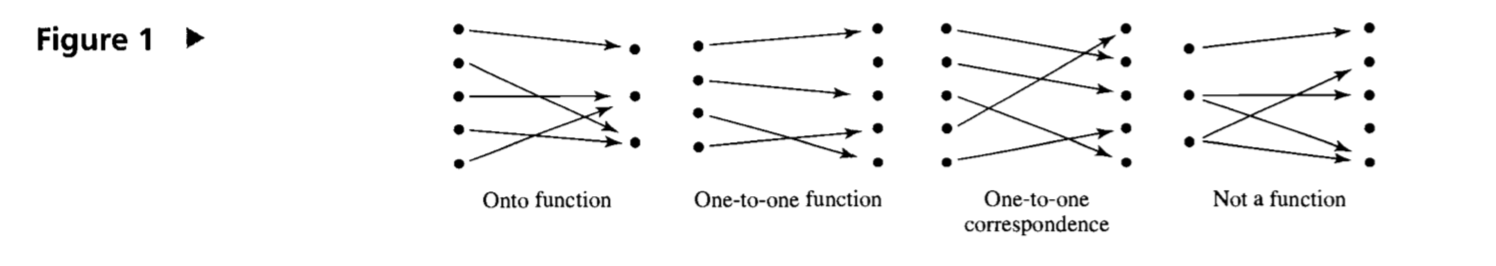
\includegraphics[width=\linewidth]{figure1_types_of_functions.png}
	\caption{types of functions}
	\label{fig:figure1}
\end{figure}
\textit{onto: every element in codomain is accounted for}\\
\textit{one-to-one: every element in domain has a unique spot in codomain}\\
\textit{one-to-one correspondence: one-to-one between domain-codomain and codomain-domain}
\end{center}

\subsection*{(a)}
\begin{center}
Are there any one-to-one functions from $S$ into $T$?\\
\hfill \break
No, this would be an onto function but doesn't meet the requirements for one-to-one.
\end{center}

\subsection*{(b)}
\begin{center}
Are there any one-to-one functions from $T$ into $S$?\\
\hfill \break
Yes. One element in $S$ will be unused.
\end{center}

\subsection*{(c)}
\begin{center}
Are there any functions mapping $S$ onto $T$?\\
\hfill \break
Yes. Some two elements from $S$ will map onto some single element in $T$.
\end{center}

\subsection*{(d)}
\begin{center}
Are there any functions mapping $T$ onto $S$?\\
\hfill \break
No, not enough elements in $T$ to fill up codomain $S$. This could be a one-to-one however.
\end{center}

\subsection*{(e)}
\begin{center}
Are there any one-to-one correspondences between $S$ and $T$?\\
\hfill \break
No, $S$ and $T$ have different number of elements.
\end{center}
%
%
\subsection*{2.}
\begin{center}
The functions sketched in Figure 3 have domain and codomain both equal to $[0,1]$\\
\begin{figure}[h!]
	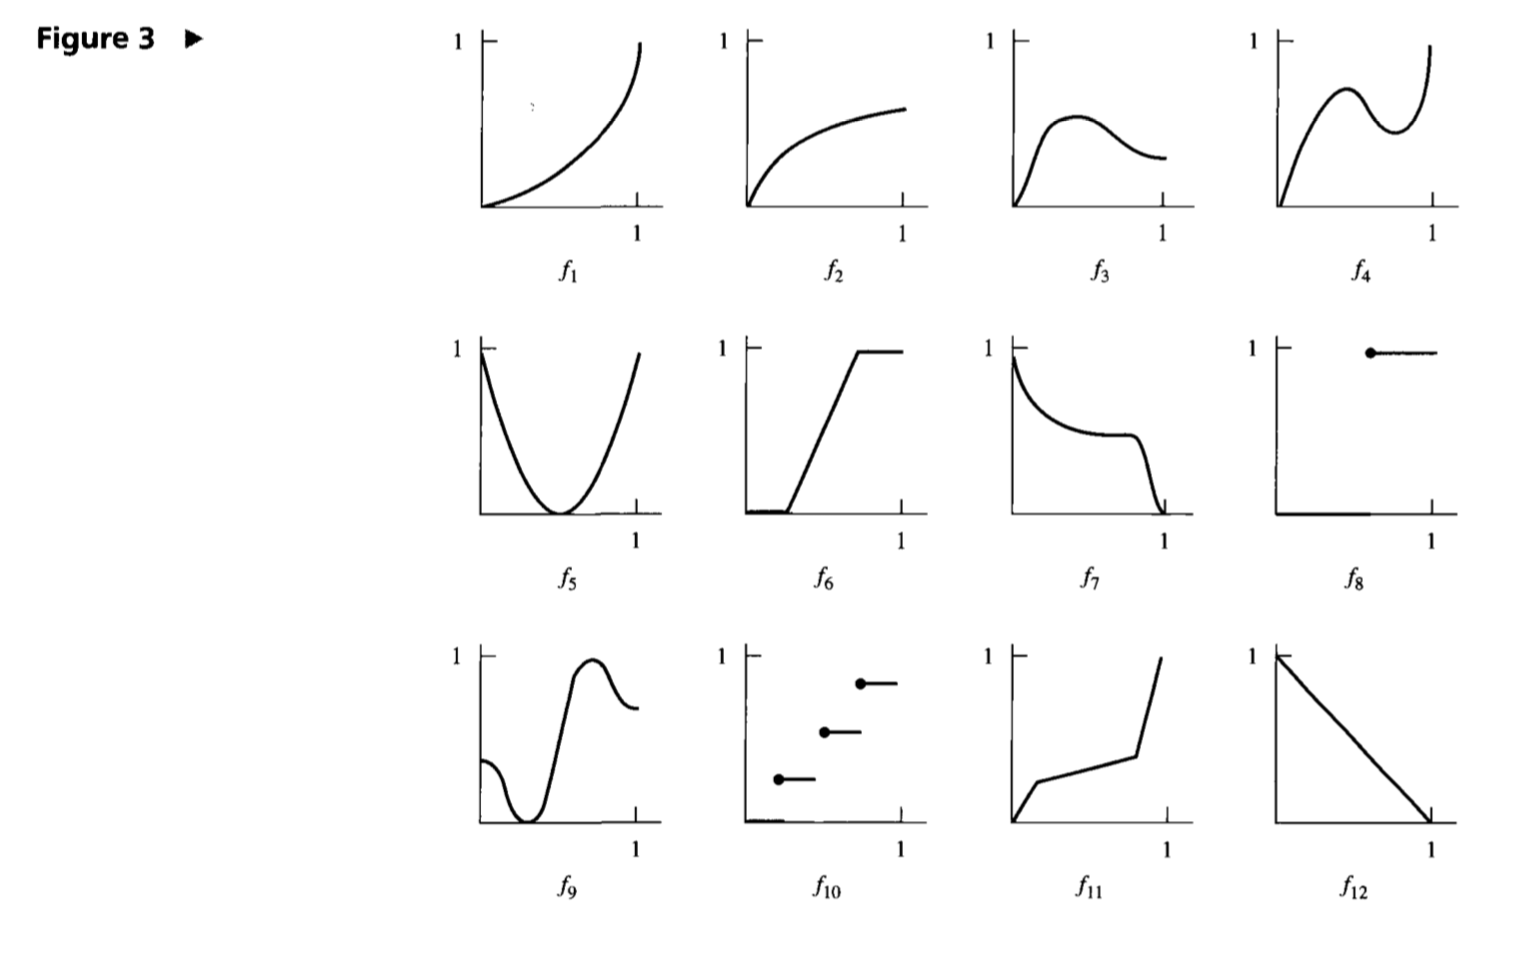
\includegraphics[width=\linewidth]{figure3.png}
\end{figure}
\textit{(TODO check with Professor about question 2)}
\end{center}

\subsection*{(a)}
\begin{center}
Which of these functions are one-to-one?\\
\hfill \break
$f_1, f_2, f_{11}, f_{12}$ because they pass the horizontal-line-test; $x$ and $y$ coordinates are not repeated on $x$ and $y$ axes.
\end{center}

\hfill \break
\subsection*{(b)}
\begin{center}
Which of these functions map $[0,1]$ onto $[0,1]$?\\
\hfill \break
$f_1, f_4, f_5, f_6, f_9, f_{11}, f_{12}$ because they fill up all the y-axis codomain elements. ($f_7$ is a bit tricky because there is a tiny gap.
\end{center}

\subsection*{(c)}
\begin{center}
Which of these functions are one-to-one correspondences?\\
\hfill \break
$f_1, f_{11}, f_{12}$ satisfy bijection requirements of both onto and one-to-one.
\end{center}
%
%
\subsection*{3.}
\begin{center}
The function $f(m,n) = 2^{m}3^{n}$ is a one-to-one function from $\mathbb{N} \times \mathbb{N} \text{ into } \mathbb{N}$.
\end{center}

\subsection*{(a)}
\begin{center}
Calculate $f(m,n)$ for five different elements $(m,n)$ in $\mathbb{N} \times \mathbb{N}$:\\
\hfill \break
$f(0,1) = 2^{0}3^{1} = 1 \cdot 3 = 3$\\
$f(2,3) = 2^{2}3^{3} = 4 \cdot 27 = 108$\\
$f(1,2) = 2^{1}3^{2} = 2 \cdot 9 = 18$\\
$f(0,2) = 2^{0}3^{2} = 1 \cdot 9 = 9$\\
$f(0,3) = 2^{0}3^{3} = 1 \cdot 27 = 27$ 
\end{center}
%
%
\subsection*{4.}
\begin{center}
Consider the following functions from $\mathbb{N} \text{ into } \mathbb{N}$:\\
$1_{\mathbb{N}}(n) = n, f(n) = 3n, g(n) = n + (-1)^{n}, h(n) = \text{min}[n, 100], k(n) = \text{max}[0, n - 5]$
\end{center}

\subsection*{(a)}
\begin{center}
Which of these functions are one-to-one?\\
\hfill \break
$1_{\mathbb{N}}(n)$\\
$f(n)$\\
$g(n)$
\end{center}

\subsection*{(b)}
\begin{center}
Which of these functions map $\mathbb{N} \text{ into } \mathbb{N}$?\\
\hfill \break
these cover all values in the $\mathbb{N}$ codomain:\\
$1_{\mathbb{N}}(n)$\\
$g(n)$
\end{center}
%
%
\subsection*{5.}
\begin{center}
Here are two "shift functions" mapping $\mathbb{N} \text{ into } \mathbb{N}$:\\
$f(n) = n + 1$ and $g(n) = \text{max}[0,n - 1] \text{ for } n \in \mathbb{N}$
\end{center}

\subsection*{(a)}
\begin{center}
Calculate $f(n)$ for $n = 0,1,2,3,4,73$:\\
\hfill \break
$f(0) = 1$\\
$f(1) = 2$\\
$f(2) = 3$\\
$f(3) = 4$\\
$f(4) = 5$\\
$f(73) = 74$
\end{center}

\subsection*{(b)}
\begin{center}
Calculate $g(n)$ for $n = 0,1,2,3,4,73$:\\
\hfill \break
$g(0) = 0$\\
$g(1) = 0$\\
$g(2) = 1$\\
$g(3) = 2$\\
$g(4) = 3$\\
$g(73) = 72$\\
\end{center}

\subsection*{(c)}
\begin{center}
Show that $f$ is one-to-one but does not map $\mathbb{N} \text{ onto } \mathbb{N}$:\\
\hfill \break
$f(n)$ always produces a unique output in codomain so it is one-to-one, but does not plot $0$ onto the codomain
\end{center}

\subsection*{(d)}
\begin{center}
Show that $g$ maps $\mathbb{N} \text{ onto } \mathbb{N}$ but is not one-to-one:\\
\hfill \break
$g(n)$ maps all numbers onto $\mathbb{N}$ codomain but is not one-to-one because $g(0) \text{ and } g(1)$ both output $0$
\end{center}

\subsection*{(e)}
\begin{center}
Show that $g \circ f(n) = n \text{ for all } n$, but that $f \circ g(n) = n \text{ does not hold for all } n$:\\
\hfill \break
$g \circ f(n)$ is essentially just $\text{max}[0,n]$, so it will output back $n$\\
$f \circ g(n)$ does not account for $0$
\end{center}
%
%
\subsection*{7.}
\begin{center}
Find the inverses of the following functions mapping  $\mathbb{R} \text{ into } \mathbb{R}$: 
\end{center}

\subsection*{(b)}
\begin{center}
$g(x) = x^{3} - 2$\\
\hfill \break
$g^{-1}(x) = \sqrt[3]{x+2}$
\end{center}

\subsection*{(c)}
\begin{center}
$h(x) = (x - 2)^{3}$\\
\hfill \break
$y = (x - 2)^{3}$\\
$\sqrt[3]{y} = x - 2$\\
$x = \sqrt[3]{y} + 2$\\
$h^{-1}(x) = \sqrt[3]{x} + 2$
\end{center}
%
%
\subsection*{9.}
\begin{center}
Show that the following functions are their own inverses:
\end{center}

\subsection*{(a)}
\begin{center}
The function $f : (0,\infty) \rightarrow (0,\infty)$ given by $f(x) = \frac{1}{x}$\\
\hfill \break
suppose $f^{-1}(x) = \frac{1}{x}$\\
let $x = 5$\\
$f(5) = \frac{1}{5}$\\
\hfill \break
$f^{-1}(f(5)) = \frac{1}{(\frac{1}{5})} = 5$
\end{center}
%
%
\subsection*{10.}
\begin{center}
Let $A$ be a subset of some set $S$ and consider the characteristic function $X_{A}$ of $A$.\\
Find $X_{A}^{-1}(1) \text { and } X_{A}^{-1}(0)$:\\
\hfill \break
$X_{A}^{-1}(1) = A$\\
\hfill \break
$X_{A}^{-1}(0) = A^{c}$
\end{center}
%
%
\hfill \break
\hfill \break
\hfill \break
\subsection*{11.}
\begin{center}
Here are some functions from $\mathbb{N} \times \mathbb{N} \text{ to } \mathbb{N}$:\\
$\text{SUM}(m,n) = m + n, \text{PROD}(m,n) = m \cdot n, \text{MAX}(m,n) = \text{max}\{m,n\}, \text{MIN}(m,n) = \text{min}\{m,n\}$
\end{center}

\subsection*{(a)}
\begin{center}
Which of these functions map $\mathbb{N} \times \mathbb{N} \text{ onto } \mathbb{N}$?\\
\hfill \break
With the right combinations, all of them could cover infinite values for $i \in \mathbb{N}$.
\end{center}

\end{document}
